\documentclass[12pt,a4paper,twoside]{book}
\usepackage{graphicx}
\usepackage{setspace} % espaciado doble para texto, simple para pies de página, subtítulos, etc.
\usepackage{natbib} % sustituto de 'hypernat' que funciona en Windows.
\usepackage[spanish]{babel}
\usepackage[utf8]{inputenc}
\usepackage{color}
\usepackage{hhline} % estilos extendidos para tablas
\usepackage{multirow}
\usepackage{subfigure}
\usepackage{acronym}
\usepackage{hyperref}
\usepackage{amsmath,amssymb}
\usepackage{fancyhdr}
\usepackage{epsfig, amsmath}
\usepackage{algorithm}
\usepackage{algorithmic}



% configuraciones generales
\hypersetup{
linktocpage=true,
colorlinks=true,
linkcolor=blue,
citecolor=blue,
}
\definecolor{Hgray}{gray}{0.6}

\newenvironment{definition}[1][Definición]{\begin{trivlist}
\item[\hskip \labelsep {\bfseries #1}]}{\end{trivlist}}

\setlength{\topmargin}{0cm}
\setlength{\textheight}{23cm}
\setlength{\textwidth}{17cm}
\setlength{\oddsidemargin}{0cm}
\setlength{\evensidemargin}{0cm}
\setlength{\headheight}{1cm}

% indica que las 'sub-sub-secciones' están numeradas y aparecen en el índice
\setcounter{secnumdepth}{3}
\setcounter{tocdepth}{2}

% configuraciones para código
\renewcommand{\algorithmicrequire}{\textbf{Entrada:}}
\renewcommand{\algorithmicensure}{\textbf{Salida:}}

%%%%%%%%%%%%
% DOCUMENTO %
%%%%%%%%%%%%
\begin{document}

\setcounter{section}{0} % Restablece el contador de sección a 0 al inicio del documento
\renewcommand{\thesection}{\arabic{section}} % Cambia el esquema de numeración de sección

% portada
\newpage
\thispagestyle{empty}

\baselineskip 2em

%\vspace*{1cm}

\centerline{
\includegraphics[width=0.6\textwidth]{images/UOC-logo}}
\begin{center}
\textsc{Universitat Oberta de Catalunya (UOC) \\
 Máster Universitario en Ciencia de Datos (\textit{Data Science})\\}

%\centerline {\pic{UOC}{4cm}}

\vspace*{1.5cm}

\textsc{\Large TRABAJO FINAL DE MÁSTER}

\vspace*{0.5cm}

\textsc{\large Área: Natural Language Processing and Visual Analytics\\}
\textsc{\large Data Mining, Graphs and Natural Language Processing}

%\textbf{\Huge VirtualTechLab Model: }

\vspace*{2.0cm}

\textbf{\Large Desarrollo de un RAG avanzado para la obtención 
de información sobre convocatorias de ayudas a empresas}

%\textbf{\large xxx subtítulo (en caso de existir) xxx}

\vspace{2.5cm}
\baselineskip 1em

\baselineskip 2em
-----------------------------------------------------------------------------\\
Autor:      José Luis Rodríguez Andreu\\
Tutor:      Diego Calvo Barreno\\
Profesor:   Josep Anton Mir Tutusaus\\
-----------------------------------------------------------------------------\\
\vspace*{1.5cm}
Barcelona, \today

\end{center}

\newpage
\pagestyle{empty}
\hfill

\newpage
% resumen
\pagenumbering{roman} 
\setcounter{page}{1} 
\pagestyle{plain}

%%%%%%%%%%%%%%%%
%%% CREDITOS %%%
%%%%%%%%%%%%%%%%
% \chapter*{Créditos/Copyright}

% Una página con la especificación de créditos/copyright para el proyecto (ya sea aplicación por un lado y documentación por el otro, o unificadamente), así como la del uso de marcas, productos o servicios de terceros (incluidos códigos fuente). Si una persona diferente al autor colaboró en el proyecto, tiene que quedar explicitada su identidad y qué hizo.

% A continuación se ejemplifica el caso más habitual, aunque se puede modificar por cualquier otra alternativa:

\vspace{1cm}

\begin{figure}[ht]
    \centering
	
\includegraphics[scale=1]{images/license.png}
\end{figure}

Esta obra está sujeta a una licencia de Reconocimiento -  NoComercial - SinObraDerivada

\href{https://creativecommons.org/licenses/by-nc-nd/3.0/es/}{3.0 España de CreativeCommons}.

%%%%%%%%%%%%%
%%% FICHA %%%
%%%%%%%%%%%%%
\chapter*{FICHA DEL TRABAJO FINAL}

\begin{table}[ht]
	\centering{}
	\renewcommand{\arraystretch}{2}
	\begin{tabular}{r | l}
		\hline
		Título del trabajo: & Desarrollo de un RAG avanzado para la obtención 
		de información sobre convocatorias de ayudas a empresas\\
		\hline
        Nombre del autor: & José Luis Rodríguez Andreu\\
		\hline
        Nombre del colaborador/a docente: & Diego Calvo Barreno\\
		\hline
        Nombre del PRA: & Josep Anton Mir Tutusaus\\
		\hline
        Fecha de entrega (mm/aaaa): & 06/2025\\
		\hline
        Titulación o programa: & Máster Universitario en Ciencia de Datos\\
		\hline
        Área del Trabajo Final: & Trabajo Fin de Máster\\
		\hline
        Idioma del trabajo: & Español\\
		\hline
        Palabras clave & LLM, RAG, AI\\
		\hline
	\end{tabular}
\end{table}

%%%%%%%%%%%%%%%%%%%
%%% DEDICATORIA %%%
%%%%%%%%%%%%%%%%%%%
\chapter*{Dedicatoria/Cita}

Breves palabras de dedicatoria y/o una cita.
%A Miguel, que lleva el nombre de un poeta valiente, y a Carmen, 

%%%%%%%%%%%%%%%%%%%
%%% Agradecimientos %%%
%%%%%%%%%%%%%%%%%%%
\chapter*{Agradecimientos}

Si se considera oportuno, mencionar a las personas, empresas o instituciones que hayan contribuido en la realización de este proyecto.

%%%%%%%%%%%%%%%%
%%% Abstract  %%%
%%%%%%%%%%%%%%%%
\chapter*{Abstract}
\addcontentsline{toc}{chapter}{Abstract}

\onehalfspacing

Texto con la síntesis del proyecto, esto es, un texto en el cual se explica de manera concisa la definición del proyecto/problema abordado, sus objetivos/métodos de resolución, y los resultados y conclusiones (no puede ser una lista, sino un texto continuo redactado de manera estructurada). Si es necesario poner una referencia en este texto, ésta será anotada a pie de la misma página. En este apartado se puede usar un lenguaje más literario y coloquial que para el resto del documento.

El Abstract se escribirá por duplicado. Una de las versiones tiene que ser \textbf{obligatoriamente en inglés}. La otra versión tiene que estar escrita en catalán o español. En caso de no escribir el resto del documento en inglés, será necesario escribir la segunda versión del Abstract en el idioma utilizado para el resto de la memoria. La palabra Abstract se cambiará por ``\textbf{Resum}'' o ``\textbf{Resumen}'' en la versión catalana y española, respectivamente. 

Extensión recomendada: 250 palabras máximo.

Como escribir un buen Abstract (en inglés):

\href{http://www.ece.cmu.edu/~koopman/essays/abstract.html}{http://www.ece.cmu.edu/~koopman/essays/abstract.html}

\vspace{1.5cm}

\textbf{Palabras clave}: Keywords del trabajo separadas por comas. Por ejemplo para este documento podrían ser Modelo, Pauta, Plantilla, Memoria, Trabajo de Final de Grado/Máster

%%%%%%%%%%%%%%%%
%%% RESUMEN  %%%
%%%%%%%%%%%%%%%%
\chapter*{Resumen}
\addcontentsline{toc}{chapter}{Resumen}

\onehalfspacing

Texto con la síntesis del proyecto, esto es, un texto en el cual se explica de manera concisa la definición del proyecto/problema abordado, sus objetivos/métodos de resolución, y los resultados y conclusiones (no puede ser una lista, sino un texto continuo redactado de manera estructurada). Si es necesario poner una referencia en este texto, ésta será anotada a pie de la misma página. En este apartado se puede usar un lenguaje más literario y coloquial que para el resto del documento.

El Abstract se escribirá por duplicado. Una de las versiones tiene que ser \textbf{obligatoriamente en inglés}. La otra versión tiene que estar escrita en catalán o español. En caso de no escribir el resto del documento en inglés, será necesario escribir la segunda versión del Abstract en el idioma utilizado para el resto de la memoria. La palabra Abstract se cambiará por ``\textbf{Resum}'' o ``\textbf{Resumen}'' en la versión catalana y española, respectivamente. 

Extensión recomendada: 250 palabras máximo.

Como escribir un buen Abstract (en inglés):

\href{http://www.ece.cmu.edu/~koopman/essays/abstract.html}{http://www.ece.cmu.edu/~koopman/essays/abstract.html}

\vspace{1.5cm}

\textbf{Palabras clave}: Keywords del trabajo separadas por comas. Por ejemplo para este documento podrían ser Modelo, Pauta, Plantilla, Memoria, Trabajo de Final de Grado/Máster
\newpage

\pagestyle{fancy}
\renewcommand{\chaptermark}[1]{ \markboth{#1}{}}
\renewcommand{\sectionmark}[1]{\markright{ \thesection.\ #1}}
\lhead[\fancyplain{}{\bfseries\thepage}]{\fancyplain{}{\bfseries\rightmark}}
\rhead[\fancyplain{}{\bfseries\leftmark}]{\fancyplain{}{\bfseries\thepage}}
\cfoot{}

% tabla de contenidos
\cleardoublepage
\phantomsection
\addcontentsline{toc}{chapter}{Índice}
\tableofcontents
% lista de figuras
\cleardoublepage
\phantomsection
\addcontentsline{toc}{chapter}{Lista de Figuras}
\listoffigures
% lista de tablas
\cleardoublepage
\phantomsection
\addcontentsline{toc}{chapter}{Lista de Tablas}
\listoftables

\thispagestyle{empty}

\pagenumbering{arabic}

\pagestyle{fancy}
\renewcommand{\chaptermark}[1]{ \markboth{#1}{}}
\renewcommand{\sectionmark}[1]{\markright{ \thesection.\ #1}}
\lhead[\fancyplain{}{\bfseries\thepage}]{\fancyplain{}{\bfseries\rightmark}}
\rhead[\fancyplain{}{\bfseries\leftmark}]{\fancyplain{}{\bfseries\thepage}}
\cfoot{}

\onehalfspacing

% capítulos del documento
\chapter{Introducción}
\label{chapter:introduccion}


%%% SECTION
\section{Descripción general del problema}

En la actualidad, los procesos de minería de datos requieren grandes cantidades de datos, que en muchas ocasiones contienen información personal y privada de usuarios o personas. Aunque se realicen procesos básicos de anonimización sobre los datos, es decir, eliminación de los nombres u otros identificadores clave, existen multitud de técnicas de re-identificación que permiten volver a identificar a un usuario dentro de este conjunto de datos. En la Figura \ref{fig:context-anoni1} se presenta un mapa donde es posible contextualizar los procesos de anonimización y re-identificación dentro de un proceso de minería de datos.

\begin{figure}
	\centering
	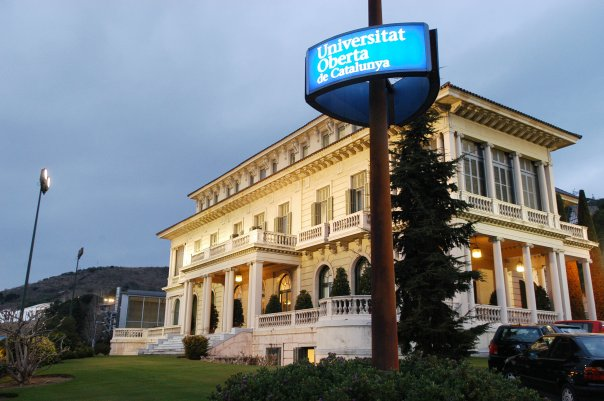
\includegraphics[width=0.6\textwidth]{figs/image1.png}
	\caption{Pie de la imagen.}
	\label{fig:context-anoni1}
\end{figure}

\subsection{Ejemplo de subsection}

Aunque se han realizado importantes avances en preservación de la privacidad en publicación de datos, tales como el modelo \textit{k}-anonymity \cite{Sweeney:2002}.

Un ejemplo de pseudo-código se puede encontrar en el Código \ref{code:RandomSwitch-1}

\begin{algorithm}
	\caption{Pseudocódigo del algoritmo \textit{Random Switch}}
	\label{code:RandomSwitch-1}
	\begin{algorithmic}
		\REQUIRE{El grafo original $G$ y el porcentaje de anonimización $p$ que se desea aplicar.}
		\ENSURE{El grafo $G$ anonimizado.}
		\STATE $num = round(G.num\_edges() * p)$
		\STATE $i = 0$
		\WHILE {$i < num$}
		\STATE {$e_{1} = G.random\_edge()$}
		\STATE $e_{2} = G.random\_edge()$
		\STATE $new\_e_{1} = (e_{1}.origen, e_{2}.origen)$
		\STATE $new\_e_{2} = (e_{1}.destino, e_{2}.destino)$
		\IF {$!G.exist(new\_e_{1})$ \AND $!G.exist(new\_e_{2})$}
		\STATE $G.add\_edge(new\_e_{1})$
		\STATE $G.add\_edge(new\_e_{2})$
		\STATE $G.delete\_edge(e_{1})$
		\STATE $G.delete\_edge(e_{2})$
		\STATE $i=i+1$
		\ENDIF
		\ENDWHILE
		\RETURN $G$
	\end{algorithmic}
\end{algorithm}

Un ejemplo de tabla se puede ver en la Tabla \ref{table:ejemplo_vertex_refi_query}

\begin{table}
	\centering{}
	\begin{tabular}{ l || c | c | l }
		\hline
		Node ID & $\mathcal{H}_{0}$ & $\mathcal{H}_{1}$ & $\mathcal{H}_{2}$ \\
		\hline
		\hline
		Alice & $\epsilon$ & 1 & \{4\}  \\
		\hline
		Bob & $\epsilon$ & 4 & \{1, 1, 4, 4\}  \\
		\hline
		Carol & $\epsilon$ & 1 & \{4\}  \\
		\hline
		Dave & $\epsilon$ & 4 & \{2, 4, 4, 4\}  \\
		\hline
		Ed & $\epsilon$ & 4 & \{2, 4, 4, 4\}  \\
		\hline
		Fred & $\epsilon$ & 2 & \{4, 4\}  \\
		\hline
		Greg & $\epsilon$ & 4 & \{2, 2, 4, 4\}  \\
		\hline
		Harry & $\epsilon$ & 2 & \{4, 4\}  \\
		\hline
	\end{tabular}
	\caption{\textit{Vertex refinement queries}.}
	\label{table:ejemplo_vertex_refi_query}
\end{table}
\newpage

\chapter{Estado del Arte}
\label{chapter:Estado del Arte}


%%% SECTION
\section{Introducción}
El objetivo de este capítulo es realizar un análisis de los diferentes avances, desarrollos y tecnologías disponibles en el ámbito de la solución planteada. 

Este análisis tiene como objetivo identificar enfoques y metodologías en distintas áreas, como la extracción de información a partir de fuentes web, el análisis y procesado de texto y el uso de técnicas de Inteligencia Artificial aplicadas al Procesamiento de Lenguaje Natural.

De esta forma se puede establecer un contexto para el problema a resolver y justificar la elección de las tecnologías y metodologías a utilizar en el desarrollo de la solución propuesta.

\section{Problemática a resolver}

La búsqueda de ayudas y subvenciones es una tarea que la mayoría de las empresas, sobre todo las que tienen menos recursos, realizan en su día a día.
Para ello, existen diferentes plataformas de ayudas a empresas, algunas nacionales y otras de carácter internacional. 
Sin embargo, esta tarea puede resultar complicada y tediosa, ya que implica una búsqueda constante de nuevas posibilidades de financiacióna través de distintas fuentes.
Además, la información sobre estas convocatorias suele estar distribuidas en diferentes fuentes, desde las propias plataformas a documentación oficial del estado.
Esto supone que a la hora de realizar una búsqueda de posibles convocatorias de financiación, se acabe con un conjunto de fuentes con diferentes estructuras y formatos.

En la mayoría de los casos, las convocatorias suelen tener asociados diferentes documentos, en su mayoría en formato PDF, los cuales pueden ser extensos, y además usan un lenguaje técnico, típico de este tipo de documentos, que dificulta su comprensión.
Esto al final supone una complicación por parte de las empresas a la hora de acceder a información clave de las convocatorias de forma mas rápida, como requisitos, plazos, presupuesto o condiciones de participación.
Estos problemas de accesibilidad y estandarización de las convocatorias de ayudas suponen una barrera de acceso importante, que reduce las oportunidades de acceso a financiación para algunas empresas, y suponen una inversión en tiempo y esfuerzo en la tarea de búsqueda y filtrado por parte de éstas

El desarrollo planteado en este proyecto pretende ser una solución a esta problemática, proporcionando una herramienta que sea capaz de identificar y extraer la documentación de las convocatorias, y aplicar técnicas de Inteligencia Artificial para extraer la información clave y dotarla de una estructura mas estandarizada, así como permitir la consulta de esta información de forma sencilla a partir de un agente conversacional.


% \section{Soluciones clásicas}


% \subsection{Plataformas de convocatorias}

% \subsection{Web Scraping}

% \subsection{Procesamiento de Lenguaje Natural}

% \section{Inteligencia Artificial Generativa}

% \subsection{Grandes Modelos del Lenguaje (LLMs)}

% \subsection{Prompt Engineering}

% \subsection{Retrieval Augmented Generation (RAG)}

% \subsection{Agentes Inteligentes}

% \section{Tecnologías y métodos actuales}

% \section{conclusiones}
\newpage

\chapter{Métodos y recursos}
\label{chapter:Métodos y recursos}


\section{Introducción}

Este capítulo presenta la metodología y las herramientas empleada en el desarrollo del proyecto, detallando cada fase de diseño, implementación y pruebas. 
Tras realizar una planificación exhaustiva y un análisis del estado del arte en el capítulo anterior, se ha adquirido un marco preciso sobre los objetivos y las etapas necesarias para alcanzar los objetivos de este proyecto. 
Con esta base sólida, se procede a estructurar y ejecutar el desarrollo del producto utilizando metodologías y recursos que se ajusten a las necesidades de automatización y procesamiento de datos que plantea el proyecto.

\subsection{Descripción general del capítulo}

El capítulo muestra un desglose de las decisiones metodológicas y técnicas que sustentan el diseño y desarrollo de la solución. 
Incluye una descripción de los recursos tecnológicos, tanto de hardware como de software, empleados para asegurar la eficiencia y precisión en el proceso de identificación y clasificación de convocatorias de ayudas. 
Cada sección aborda de manera específica las técnicas y herramientas implementadas en cada fase del proyecto, desde la recopilación de datos con el extractor de ayudas, la generación de datos estructurados con el bloque de procesamiento, y la construcción de la herramienta de consulta de información basada en un sistema conversacional basado en agentes inteligentes.

\subsection{Importancia del diseño, desarrollo e implementación en la investigación}

El desarrollo de una solución automatizada para sintetizar y recuperar información de convocatorias es esencial en un entorno con abundancia de datos y formatos diversos. 
Un diseño eficiente asegura que cada componente cumpla su función, maximizando la precisión y minimizando redundancias. 
La implementación adapta técnicas de recuperación de información y procesamiento de lenguaje natural basadas en Inteligencia Artificial Generativa, del estado del arte a las necesidades del proyecto, mientras que una metodología ágil permite ajustes continuos y mejora constante.
Este capítulo describe los métodos y recursos que sustentan la construcción de la solución, transformando la planificación teórica en un producto funcional capaz de procesar grandes volúmenes de datos y facilitar su análisis para entidades específicas.

\section{Objetivos y Competencias}

El propósito de esta sección es detallar los objetivos específicos de la fase de desarrollo e implementación de la solución, y las competencias técnicas y metodológicas necesarias para cumplir con dichos objetivos. 
Estos aspectos son fundamentales para asegurar que cada etapa del proyecto esté alineada con los resultados esperados y que los participantes en el desarrollo cuenten con las habilidades necesarias para abordar los desafíos que puedan surgir.


\subsection{Objetivos específicos de esta fase del proyecto}

Los objetivos de la fase de desarrollo e implementación son los siguientes:

\begin{itemize}
    \item \textbf{Implementación de un sistema automático de extracción de datos de ayudas}: 
    Desarrollo de una herramienta basada en web scraping para la extracción de información.
    Esta herramienta es modular, cada uno de estos módulos está adaptadoa una fuente de convocatorias específica.
    La herramienta navega por el sitio web, identifica las diferentes convocatorias disponibles y extrae la información necesaria, como el texto resumen de la ayuda, la ficha técnica, y los documentos asociados a la convocatoria.
    \item \textbf{Desarrollo de un módulo de procesamiento de datos}: 
    Este módulo carga las fuentes de datos asociadas a cada ayuda y las procesa mediante técnicas de extracción basadas en IA Generativa.
    El objetivo es extraer diferentes parámetros de las fuentes de datos y obtener como resultado un conjunto de datos estructurados en formato tabla.
    \item \textbf{Desarrollo de un módulo de construcción de bases de datos}:
    Este módulo parte de las fuentes de datos originales y de los datos estructurados y contruye una base de datos documental y una base de datos estructurados.
    Mientras que en este caso, la base de datos estructural se crea de manera directa, para la base de datos documental es necesario implemental un bloque de procesamiento, donde los diferentes documentos se dividen en chunks y se generan sus correspondientes embeddings.
    \item \textbf{Implementación de una aplicación RAG mediante técnicas avanzadas}:
    Construcción de una solución de recuperación de información basada en un RAG multiagente, donde a través de lenguaje natural pueden generarse consultas de datos tanto a la base de datos estructurada como a la documental.
    \item \textbf{Implementación de una aplicación web para el uso del sistema multiagente como asistente conversacional}:
    Construcción de una pequeña interfaz de chat para la explotación de la herramienta de recuperación de información.
\end{itemize}

Estos objetivos son claves para asegurar que el sistema cumpla con los requisitos del proyecto y
proporcione una herramienta robusta y confiable para la identificación y análisis de convocatorias de
ayudas.



\subsection{Competencias técnicas y metodológicas requeridas}

Para la implementación de la solución de este proyecto, es necesario estar capacitado en una serie de competencias técnicas, tanto en el ámbito del desarrollo de software como en relación a diferentes técnicas de Inteligencia Artificial Generativa, Agentes inteligentes y frameworks específicos.

\begin{itemize}
    \item \textbf{Desarrollo de sistemas de captura de datos basados en web scraping}:
    Se requiere conocimiento y experiencia en herramientas y frameworks de scraping para la extracción de datos en multiples entornos web, como son el caso de BeautifulSoup y Selenium.

    \item \textbf{Desarrollo de sistemas de procesamiento de datos}:
    Conocimiento en implementación de pipelines de extracción, transformación y carga de datos. 
    Conocimiento de las principales herramientas de tratamiento de datos dentro del ecosistema Python (Numpy, Pandas, sqlalchemy).
    
    \item \textbf{Implementación de sistemas basados en Inteligencia Artificial Generativa}:
    Es necesaria una base de Procesamiento de Lenguaje Natural, que permita entender el funcionamiento de los Grandes Modelos del Lenguaje y las diferentes aplicaciones que se pueden construir con éstos.
    Se requiere, además, conocimiento de las diferentes opciones a emplear en cuanto a modelos del lenguaje, arquitecturas de uso, y vectorización de texto mediante embeddings (Prompt engineering, Retrieval Augmented Generation, Data Extraction, etc).
    
    \item \textbf{Frameworks de orquestación de soluciones basadas en LLMs y Agentes Inteligentes}: 
    Partiendo del punto anterior, es necesario el uso de frameworks específicos de IA generativa, los cuales permiten simplificar y normalizar el uso de estas herramientas. 
    Frameworks como LangChain y LanGpraph permiten implementar soluciones estandarizadas y funcionales con cualquier tipo de arquitectura, desde fuentes de datos a uso de diferentes modelos del lenguaje.
    También permiten la construcción de grafos de procesamiento donde se pueden implementar diferentes agentes, cada uno con una función específica. 
    
    \item \textbf{Bases de datos relacionales y vectoriales}: 
    Se requiere conocimientos en diseño y gestión de bases de datos relacionales para el almacenamiento y la información estructurada generada por el sistema.
    Así mismo, se requieren conocimientos en bases de datos vectoriales (FAISS, Choma, etc) para el almacenamiento y consulta de los diferentes documentos, y sus embeddings asociados.

    \item \textbf{Implementación de interfaz gráfica}: 
    Capacidad para implementar una interfaz gráfica que permita el uso de la aplicación mas allá de una consola de comandos.   
\end{itemize}

Estas competencias son fundamentales para abordar los objetivos de este proyecto, y obtener como resultado un sistema robusto y eficiente que sea capaz de cumplir las necesidades establecidas. 


\section{Diseño del sistema}

La solución desarrollada está estructurada en tres bloques principales: El sistema de extracción, el módulo de procesamiento, y la aplicación de consulta.
Estos tres módulos trabajan en conjunto para formar un sistema automatizable que extraiga información a partir de diferentes fuentes de convocatorias, las procese debidamente, y las incluya en el asistente conversacional de consulta.

\subsection{Arquitectura general}

La arquitectura general del sistema se compone de los siguientes módulos principales:

\begin{itemize}
    \item \textbf{Módulo de Extracción de Datos}:
    La principal funcionalidad de este módulo es la búsqueda, en cada uno de los portales de convocatorias incluidos en el sistema, de diferentes convocatorias de ayudas disponibles.
    Para cada ayuda encontrada, el sistema identifica diferentes fuentes de datos necesarias: Texto resumen de la convocatoria, ficha técnica, y documentos (generalmente pdf) asociados a la convocatoria o a sus bases.
    Este módulo se basa principalmente en herramientas de web scraping, específicamente BeautifulSoup para la intepretación de código HTML, y Selenium para la navegación por sitios web dinámicos.
    Además de la extracción, también implementa una pequeña sección de preprocesamiento, para construir diferentes documentos de formato markdown para el texto plano extraido del sitio web, así como la descarga correcta de los documentos pdf, y la organización de estos documentos.

    \item \textbf{Módulo de Procesamiento de Datos}:
    Este módulo implementa un flujo de procesamiento basado en técnicas de procesmaiento de datos estandar, combinadas con técnicas basadas en IA generativa para la extracción de un conjunto de parámetros específicos para cada ayuda.
    Internamente se han empleado diferentes técnicas implementadas desde el framework LangChain: Prompt Engineering para la construcción de prompts robustos de extracción de datos, cadenas de procesamiento de LangChain para la implementación de pipelines, y técnicas de RAG para la extracción de información de documentos mas extensos.
    
    \item \textbf{Módulo de Construcción de Bases de Datos}:
    Este módulo parte de los datos de convocatorias en crudo y de los datos estructurados extraidos del módulo anterior, y los integra en las diferentes bases de datos del sistema.
    En este caso, la integración de los datos estructurados se realiza en una base de datos SQL, mientras que los documentos pasan por un proceso de segmentación en chunks, generación de embeddings y integración en una base de datos vectorial.

    \item \textbf{Sistema de Recuperación de Información (RAG multiagente)}:
    Esta aplicación consiste en una arquitectura RAG multiagente avanzada, donde dispone de la base de datos vectorial y la base de datos SQL como fuentes documentales, a las cuales puede acceder, realizar búsquedas y extraer información contextual en base a las consultas realizadas.
    Está construida desde los frameworks LangChain y LanGraph y permite enlazar un Gran Modelo del Lenguaje a las fuentes de datos.
    \item \textbf{Interfaz de Usuario}:
    Se ha desarrollado una interfaz de usuario sencilla empleando la librería Streamlit, la cual permite levantar en pocas líneas de código una aplicación gráfica a modo de chatbot, e interactuar con el RAG multiagente.
\end{itemize}



\subsection{Flujo de trabajo del sistema}

La solución planteada está diseñada para que se pueda ejecutar de forma eficiente siguiendo un flujo de trabajo, integrando todo el proceso ETL que supone la búsqueda de convocatorias con la herramienta de consulta.
Los pasos clave del flujo de trabajo son los siguientes:

\begin{itemize}
    \item \textbf{Extracción de datos}:
    El módulo de extracción emplea web scraping para la búsqueda y descarga de las diferentes ayudas encontradas, siguiendo un algoritmo de búsqueda específico para cada portal de ayudas, ya que éste está ligado al formato de la página web.

    \item \textbf{Procesamiento de datos}:
    A partir de los datos en crudo se generan dos flujos de trabajo: El primero consiste en la extracción de parámetros y variables específicas de las fuentes de cada ayuda, mientras que el segundo realiza un preprocesado de los documentos, los divide en chunks y genera sus embeddings asociados.

    \item \textbf{Carga en las bases de datos}: A partir de los datos procesados, se actualizan tanto la base de datos SQL como la vectorial, además de generar los ficheros binarios necesarios para la aplicación RAG.

    \item \textbf{Integración de la aplicación RAG con las bases de datos}:
    Una vez han sido actualizadas las bases de datos, la aplicación RAG ya tiene acceso al contenido actualizado.
\end{itemize}

La solución está planteada de forma que se ejecuten periódicamente los tres primeros pasos para mantener actualizadas las bases de datos.


\section{Tecnologías y herramientas}

En esta sección se describen las herramientas y tecnologías seleccionadas para la implementación del sistema y el desarrollo de cada módulo.
Las tecnologías empleadas han sido seleccionadas en base a su eficacia, su posición dentro de cada grupo de tecnologías específicas que se emplean en el mercado, y su facilidad para implementar en un entorno local con pocos recursos.


\subsection{Tecnologías seleccionadas}

A continuación, se detallan las tecnologías clave empleadas:

\begin{itemize}
    \item \textbf{Python}: Se ha seleccionado Python como lenguaje de desarrollo principal por razones obvias: Es el lenguaje de programación mas empleado en el campo de la Ciencia de Datos y la Inteligencia Artificial. Esto implica que la gran mayoría de herramientas, frameworks y librerías de estos ámbitos están disponibles en Python. Esto, junto a la simplicidad que presenta el propio lenguaje, facilita y simplifica el desarrollo de cualquier solución de esta índole.
    
    \item \textbf{Beautifulsoup y Selenium}: Para la extracción de datos de sitios web, se utilizan BeautifulSoup y Selenium. 
    BeautifulSoup permite analizar y manipular la estructura HTML de las páginas, mientras que Selenium se emplea para interactuar con sitios web que requieren carga dinámica de contenido. 
    Juntos, estos paquetes permiten implementar un sistema de extracción robusto, capaz de navegar y extraer información relevante de manera eficiente.
    
    \item \textbf{SQLite}: SQLite es un sistema de gestión de bases de datos relacional embebido, de código abierto, que implementa una base de datos transaccional autocontenida, sin necesidad de un servidor dedicado. 
    Se caracteriza por su ligereza, portabilidad y facilidad de integración en aplicaciones de escritorio, móviles y sistemas embebidos. 
    SQLite almacena los datos en un único archivo en disco, lo que simplifica la gestión y el despliegue, mientras que soporta operaciones ACID, garantizando la integridad y fiabilidad de los datos. 
    Su arquitectura libre de configuración lo convierte en una solución óptima para aplicaciones que requieren una base de datos local con bajo consumo de recursos y alta eficiencia en operaciones de lectura y escritura.
    
    \item \textbf{FAISS} (Facebook AI Similarity Search): es una librería de código abierto desarrollada por Meta AI, diseñada para realizar búsquedas eficientes de vectores de alta dimensión, optimizando la recuperación de similitudes en grandes volúmenes de datos. 
    FAISS permite construir índices que soportan tanto búsquedas exactas como aproximadas, utilizando técnicas avanzadas de cuantización y particionamiento, lo que la hace especialmente adecuada para aplicaciones de recuperación de información. 
    Gracias a su arquitectura optimizada para CPU y GPU, FAISS ofrece un alto rendimiento en tareas de búsqueda a gran escala, permitiendo gestionar millones o incluso miles de millones de vectores con tiempos de respuesta reducidos y consumo eficiente de recursos.
    
    \item \textbf{FAISS - BM25}: La extensión de FAISS para soporte de modelos de recuperación basados en términos, como BM25 (Best Matching 25), permite combinar las capacidades de búsqueda vectorial de alta dimensión con técnicas clásicas de recuperación de información basadas en el modelo probabilístico BM25. 
    Esta integración posibilita la indexación y búsqueda eficiente de documentos textuales, aplicando BM25 sobre representaciones de términos discretos mediante mecanismos optimizados dentro del entorno de FAISS. 
    De esta manera, se obtiene una solución híbrida que aprovecha la eficiencia y escalabilidad de FAISS para búsquedas aproximadas, al tiempo que incorpora un modelo estadístico robusto y ampliamente probado para la recuperación de documentos basada en la relevancia por frecuencia de término e inverso de frecuencia documental (TF-IDF mejorado). 
    Esta capacidad permite diseñar sistemas de búsqueda más versátiles y precisos en escenarios donde se requiere combinar búsquedas semánticas con búsquedas léxicas tradicionales.
    
    \item \textbf{LangChain}: Es un framework de código abierto orientado a la creación de aplicaciones que integra Grandes Modelos del Lenguaje con fuentes de datos externas, herramientas y flujos de trabajo complejos. 
    Su arquitectura modular permite orquestar cadenas de llamadas a modelos, agentes, memorias y herramientas externas, facilitando la construcción de aplicaciones conversacionales, asistentes virtuales, sistemas de pregunta-respuesta sobre documentos y soluciones de razonamiento avanzado. 
    LangChain proporciona abstracciones de alto nivel para gestionar la interacción dinámica entre modelos, usuarios y datos, soportando integraciones con bases de datos vectoriales, motores de búsqueda, APIs y sistemas de recuperación de información. 
    Esto permite desarrollar soluciones contextuales, reactivas y personalizadas que aprovechan el potencial de los LLMs combinándolos con lógica de negocio, flujos condicionales y datos propios de la organización.
    
    \item \textbf{LanGraph}: Es una extensión de código abierto para LangChain que permite modelar y ejecutar flujos conversacionales complejos mediante grafos de estado dinámicos. 
    Basado en el paradigma de máquinas de estado y grafos dirigidos, LangGraph proporciona una abstracción flexible para definir nodos que encapsulan agentes, cadenas de modelos de lenguaje, funciones o cualquier unidad lógica, permitiendo controlar de manera explícita las transiciones entre estados en función de la entrada, el contexto o condiciones personalizadas. 
    Esta capacidad resulta especialmente útil para construir aplicaciones conversacionales multi-turno, flujos de trabajo ramificados, agentes colaborativos y sistemas de toma de decisiones basados en LLMs. 
    Además, LangGraph permite la reutilización, trazabilidad y depuración de flujos, facilitando el desarrollo de sistemas robustos, auditables y adaptables a escenarios empresariales complejos donde se requiere control granular del comportamiento conversacional y de los procesos impulsados por inteligencia artificial.
    
    \item \textbf{Streamlit}: Es un framework de código abierto orientado al desarrollo ágil de interfaces web interactivas para aplicaciones de ciencia de datos, machine learning y visualización de información. 
    Diseñado con un enfoque declarativo y minimalista, Streamlit permite a los desarrolladores crear aplicaciones web funcionales utilizando exclusivamente Python, sin necesidad de conocimientos avanzados en desarrollo frontend. 
    La plataforma facilita la integración directa con librerías populares como Pandas, Matplotlib, Plotly o TensorFlow, permitiendo desplegar dashboards interactivos, formularios y visualizaciones en tiempo real con mínima complejidad. 
    Además, Streamlit soporta actualizaciones reactivas y dinámicas del contenido en función de la interacción del usuario, habilitando la creación de prototipos rápidos, demostradores y herramientas de toma de decisiones basadas en datos de manera eficiente y escalable.
\end{itemize}



\subsection{Implementación del módulo de extracción de datos}

Este módulo ha sido el primero en desarrollarse, y su función principal es la búsqueda y recopilación de datos de plataformas en diversas plataformas.
Está diseñado con una arquitectura modular, en la cual se pueden integrar diferentes módulos asociados a cada fuente de convocatorias. 


\begin{itemize}
    \item \textbf{Fuentes de datos}: En principio, se ha implementado el módulo asociado a la plataforma CDTI, pudiendo integrarse diferentes módulos posteriormente.
    \item \textbf{Extracción de datos y documentos}: Para la extracción de datos intrínsecos de los sitios web, se emplea la combinación de BeautifulSoup con Selenium.
    Mientras que Beautifulsoup permite la busqueda y extracción de información a partir de las etiquetas HTML, Selenium permite interactuar con páginas que requieren carga dinámica, como botones, tablas, o bloques de texto cargados mediante Javascript.
    Adicionalmente, se identifican posibles enlaces a documentación en formato PDF.
    \item \textbf{Preprocesamiento de datos}: Para cada página asociada a una convocatoria, se extraen diferentes bloques de texto o datos, los cuales son sometidos  auna limpieza inicial, eliminando duplicados, normalizando el formato e integrando diferentes bloques para formar un documento de texto en formato Markdown.
\end{itemize}



\subsubsection{Implementación del módulo específico para CDTI}

El módulo asociado a CDTI sigue el siguiente flujo de trabajo:

\begin{itemize}
    \item En primer lugar se identifica la Matriz de ayudas. El portal web de CDTI presenta una tabla con diferentes ayudas disponibles según siferentes categorías. Como primer paso, el módulo extrae esa matriz de ayudas junto a los enlaces correspondientes.
    \item Para cada ayuda disponible en la matriz de ayudas, El módulo analiza su página principal, e identifica los siguientes elementos:
    \begin{itemize}
        \item Bloque de resumen de la ayuda.
        \item Ficha técnica.
        \item Enlaces a documentación.
        \item Posibles subpáginas.
    \end{itemize}
    \item En el caso que existan subpáginas, entra en ellas y repite el proceso de extracción.
    \item En el caso que existan enlaces a documentación, descarga el documento en el directorio local correspondiente mediante el comando Start-BitsTransfer de Powershell.
    Tras haber testeado diferentes métotos de descarga desde Python, esta ha sido la única solución desde Windows que permitía extraer el documento pdf correctamente. 
    \item Una vez identificados todos los bloques de texto necesarios, pasan por un preprocesado inicial para generar tres documentos en formato markdown:
    \begin{itemize}
        \item Description: Documento con el texto resumen y/o introductorio de la ayuda.
        \item Card: Ficha técnica de la ayuda.
        \item Metadata: Enlaces a documentación.
    \end{itemize}
\end{itemize}


\begin{figure}[h]
	\centering
	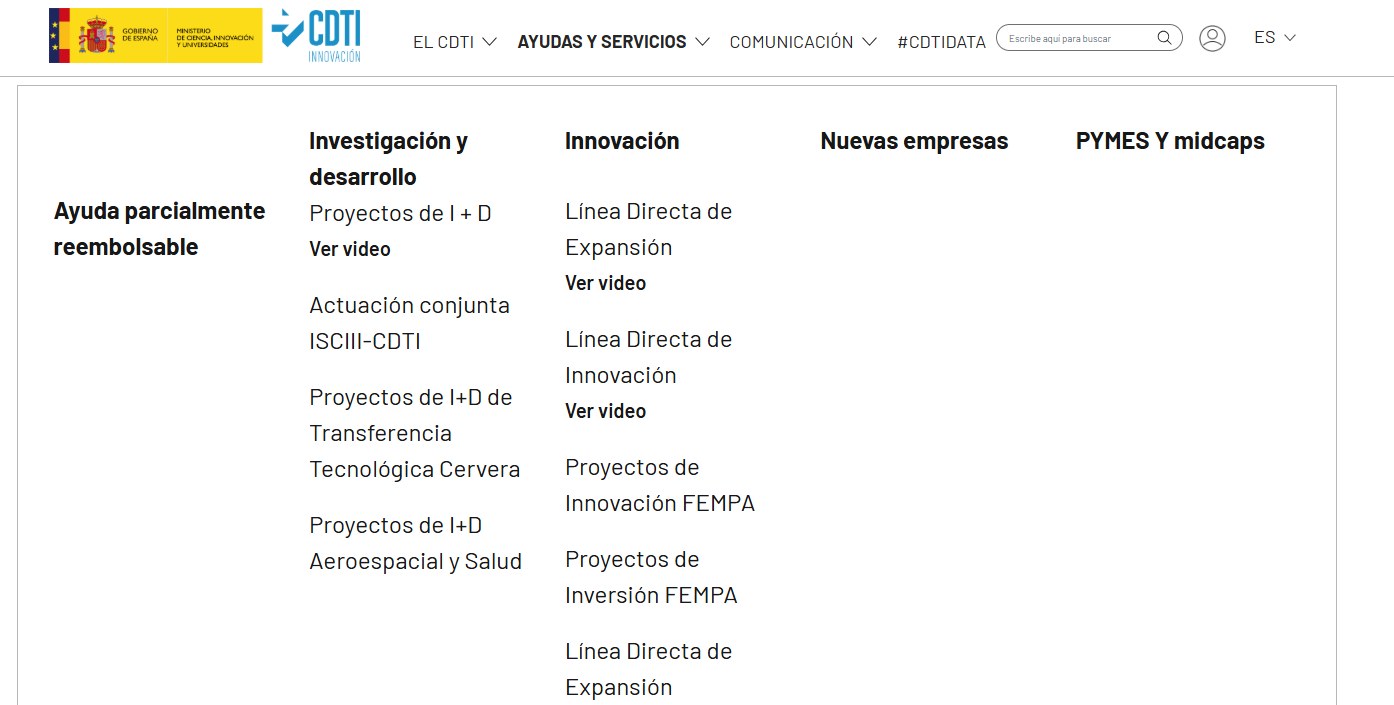
\includegraphics[width=0.8\textwidth]{figs/cdti_matrix.png}
	\caption{Matriz de ayudas del CDTI}
	\label{fig:context-anoni1}
\end{figure}


Tras la ejecución del módulo, obtenemos un directorio local para cada ayuda con los tres documentos markdown y los pdf asociados a la ayuda.


\subsection{Implementación del módulo de procesamiento de datos}


\subsection{Implementación del módulo de construcción de las bases de datos}


\subsection{Implementación del RAG multiagente}



\section{Recursos utilizados}


\subsection{Hardware y configuración del entorno}


\subsection{Software, frameworks y librerías}


\subsection{Almacenamiento de datos}



\newpage

% \chapter{Resultados}
\label{chapter:Resultados}


%%% SECTION

\section{Resultados}

Describa los resultados obtenidos utilizando la metodología descrita anteriormente.

% \newpage

% \chapter{Conclusiones y trabajo futuro}
\label{chapter:Conclusiones y trabajo futuro}


%%% SECTION

\section{Conclusiones y trabajo futuro}


\subsection{Resúmen del trabajo realizado}

En este proyecto se ha desarrollado una solución completa para la gestión, análisis y explotación de convocatorias de ayudas e empresas, donde se han combinado técnicas de extracción de datos web, técnicas de procesamiento del lenguaje natural mediante Grandes Modelos del Lenguaje, y de explotaciónd e la información mediante agentes inteligentes.
Los resultados obtenidos muestran que el sistema es capaz de explotar la información obtenida mediante consultas en lenguaje natural, realizando búsquedas tanto sobre fuentes documentales como datos estructurados.
Se destacan las siguientes características:

\begin{itemize}
    \item La solución sigue una arquitectura basada en módulos, por lo que es fácilmente escalable para incluir nuevas fuentes de datos.
    \item La combinación de bases de datos relacionales y vectoriales permiten realizar búsquedas eficientes, dotando al sistema de capacidad para responder consultas de índole mas cuantitativa sobre el conjunto de ayudas.
    \item El empleo de los frameworks LangChain y LanGraph permiten diseñar un sistema agnóstico a los modelos del lenguaje utilizados, así como a las bases de datos. La solución permite reemplazar los diferentes servicios empleados por otros de la misma índole y seguir funcionando sin problemas.
    \item El uso de LLMs como servicio desde Azure, y las bases de datos empleadas permiten la ejecución de la solución en entornos con bajos recursos, sin necesidad de una GPU para la ejecución de las llamadas a los modelos y embeddings.
\end{itemize}

\subsection{Lecciones aprendidas}

El desarrollo de esta solución ha supuesto un aprendizaje en diversos aspectos:

\begin{itemize}
    \item Se ha mejorado la comprensión y el uso de técnicas basadas en IA generativa y grandes modelos del lenguaje.
    \item Se ha obtenido una imagen global de como funcionan los frameworks LangChain y LanGraph, y como estos se interconectan con distintas opciones de fuentes de datos y modelos.
    \item El desarrollo ha estado marcado por el uso de buenas prácticas en el ámbito del desarrollo de software, avanzando mas allá de los típicos notebooks empleados en ciencia de datos y diseñando una aplicación completa.
    \item Se han revisado y testeado diferentes metodologías y arquitecturas dentro del Retrieval Augmented Generatión, así como el funcionamiento de los sistemas basados en agentes inteligentes.
\end{itemize}

\subsection{Mejoras y trabajo futuro}

La solución planteada en el proyecto es funcional y da unos resultados acordes a las necesidades del proyecto.
Sin embargo, hay ciertos puntos en los que podría mejorarse esta solución a nivel global:

\begin{itemize}
    \item Actualmente está limitada a un único portal de ayudas (CDTI). 
    Sin embargo, el diseño modular de la solución permitiría integrar fácilmente nuevas fuentes de datos en un futuro.
    \item La infraestructura de bases de datos es sencilla, de forma que pueda emplearse en local sin demasiada dificultad y sin necesidad de recursos computacionales elevados.
    Como propuesta de de mejora, se sugiere el empleo de servicios mas completos y profesionales, como por ejemplo PosgreSQL o similares para los datos estructurados, y otras opciones en cuanto a bases de datos vectoriales, como PGVector o Qdrant. 
    \item En cuanto al uso de los frameworks LangChain y LanGraph, comentar que el desarrollo empleado y las funcionalidades implementadas son funcionales, pero se contempla la posibilidad de emplear un diseño y una arquitectura mejorada, en base a los frecuentes cambios y mejoras que se implementan en estos frameworks.
    \item Del mismo modo, recientemente está cobrando fuerza en el campo de la IA generativa el concepto de MCP (Model Context Protocol). 
    Es un estándar abierto que funciona como un "USB-C" para modelos de IA, permitiendo conectar de forma uniforme cualquier modelo a múltiples fuentes de datos y herramientas externas. 
    En lugar de crear integraciones punto a punto entre cada modelo y cada servicio, MCP reduce la complejidad permitiendo a los modelos y herramientas comunicarse mediante un único protocolo común. 
    Utiliza JSON-RPC 2.0 para enviar solicitudes y recibir respuestas; así, las aplicaciones IA (clientes MCP) invocan funciones en servidores MCP que adaptan APIs, bases de datos o sistemas de archivos. 
    Los desarrolladores pueden desplegar servidores MCP para servicios como GitHub, Slack o una base de datos, y los agentes de IA eligen y llaman a estas funciones durante la generación de contenido. 
    \item Como último aporte en cuanto a mejoras, queda comentar que la solución actualmente no es 100\% reproducible, por lo que aplicar ciertas capas de abstracción en diferentes módulos, y complementar con una arquitectura de contenedores daría lugar a una aplicación agóstica del sistema operativo y completamente reproducible.
\end{itemize}

Con estas líneas de desarrollo, la solución puede seguir en evolución, con el objetivo de ganar robustez y mayor adaptabilidad a las necesidades del problema inicialmente planteado en el proyecto.
% \newpage

% \chapter{Glosario}
\label{chapter:Glosario}


%%% SECTION

\section{Glosario}

Definición de los términos y acrónimos más relevantes utilizados en este informe.

% \newpage


% bibliografía
\addcontentsline{toc}{chapter}{Bibliografía}
\bibliographystyle{plain}
\bibliography{referencias}

% \newpage
% \chapter{Anexos}
\label{chapter:Anexos}


%%% SECTION
\newpage
\section{Anexos}



Lista de secciones que son demasiado largas para ser incluidas en el cuerpo del informe y que son autocontenidas.


% \section{Anexos}

% Lista de secciones que son demasiado largas para ser incluidas en el cuerpo del informe y que son autocontenidas.

\end{document}
